\documentclass[sigconf]{acmart}
\begin{document}

\title{The Ethics of Pegasus Spyware and State-Sponsored Surveillance in the Interest of National Security}
\author{Roman Marquez-Twisdale}
\email{r.marqueztwisdale@digipen.edu}

\date{Today}
\maketitle

\section{Background Information}
Throughout this paper we will discuss the use of spyware for population surveillance in the interests of national security. Specifically, we will discuss the use of Pegasus, a piece of spyware developed by the NSO group, a for-profit Israeli cyber-arms organization and we will analyze investigations into the NSO group and Pegasus. We will attempt to reason about the ethics surrounding the use of Pegasus and dive deep into its technical abilities.
\subsection{NSO Group}
The NSO group developed the spyware known as Pegasus. To the NSO group, its success is their success. Co-founded in 2010 by two friends in high school, they specialized in hacking mobile devices from the start. “As the devices spread across the planet, governments eager to listen in came calling.” ~\cite{used_first(7)} The NSO group grew quickly with the new attention. As a major player in the spyware market, with dozens of clients and over 700 employees, their income has reached levels of around \$250 million annually as of 2018.
\subsection{Nation State Governments}
As mentioned in the previous subsection, the customers of NSO, and consumers of Pegasus are nation state governments. These governments are allegedly purchasing such a product to help ensure greater national security for themselves. Exactly what national security means will be discussed in the ethical analysis portion of this paper. National state governments can benefit from the use of Pegasus to support their interests but are also at risk of such a tool being used by their enemies.
\subsection{Nation State Populations}
The NSO group’s product targets smart mobile devices. As such, it is not a leap to say that Pegasus targets all people living in developed regions of the world. The populations of all nation states are in the crosshairs of this technology. To these populations, spyware can once again be a benefit, constraint, or outright danger depending on who you are.
\subsection{Journalists}
Journalists are a part of the world’s population, but their relationship with surveillance is unique. It is the job of a journalist to surveil the world around them, record what they see, and report any findings of consequence to organizations that will help share their findings so that society may have a better chance of recognizing and managing harmful forces. It is usually the case that journalists target and expose entities that would rather not be in the public’s eye. A successful journalist must sometimes operate unseen. Surveillance directly counters the need to be unseen. From a journalist’s perspective, Pegasus is a harmful force.
\section{Current Event Analysis}
After the NSO group started selling their first version of Pegasus, the company has been on the radar of most journalists. Especially after Edward Snowden’s whistle blowing in 2013 which exposed a similar system employed by US intelligence agencies, mass surveillance has been a hot topic. And after the assassination of a Saudi journalist in Turkey which many thought Pegasus played a role in, the NSO group has been in a very uncomfortable spotlight. The main investigation we will focus on, The Pegasus Project, started after a leaked list of roughly 50,000 phone numbers fell into the hands of a few prominent media organizations. “Forbidden Stories, a Paris-based nonprofit media organisation, and Amnesty International initially had access to the leaked list and shared access with media partners as part of the Pegasus project, a reporting consortium.” ~\cite{used_second(4)} This list of phone numbers is believed to be a list of targets for the Pegasus spyware. After receiving this list, various media partners of Forbidden Stories and Amnesty International became suspicious of the NSO group. At this point the investigation had begun, and the motivation to figure out exactly what impact Pegasus was having on the world grew quickly. The Pegasus Project consists of 17 media organizations from 10 different countries.
\section{Response to the Event}
After the birth of the Pegasus Project, evidence against NSO group started to build as the newly discovered list of roughly 50,000 phone numbers was analyzed. “From this list, an analysis of 67 smartphones provided evidence that 37 belonging to journalists, human rights activists, business executives, and two women close to Saudi activists and Washington Post columnist Jamal Khashoggi were targeted or successfully infected by the Pegasus spyware.” ~\cite{used_third(2)} These discoveries fueled the fire behind the investigation, but the fate of Khashoggi played an especially impactful role in exposing the dangers of Pegasus. Before the investigation, in 2018, a close friend of Khashoggi took NSO to court with the belief that their spyware was instrumental in his murder.
\subsection{WhatsApp}
“The following year, Amnesty International and even Facebook joined the growing list of plaintiffs after more than 1,500 people’s phones were revealed to have been targeted through a security flaw in the encrypted messaging service WhatsApp.” ~\cite{used_fourth(3)} Of those prosecuting NSO group, one of the most significant rulings was a fine of \$167 million to compensate WhatsApp for compromising the platform’s promise of secure communication. This was reduced to \$4 million alongside the addition of an official ban which prevents NSO group from hacking WhatsApp to enable its spyware’s functionality. NSO group’s ability to function was significantly impaired due to this settlement. “NSO has previously argued that an injunction preventing it from going after WhatsApp "would put NSO’s entire enterprise at risk" and "force NSO out of business," according to the judgment.” ~\cite{used_fifth(8)} In addition to financial reparations, various actions were taken by global authorities which have the result of restricting NSO group’s ability to operate.
\subsection{Entity and Sanctions Lists}
In the US, the Commerce Department’s Bureau of Industry and Security (BIS) added NSO to the Entity list, a collection of “foreign persons, entities, or governments” ~\cite{used_sixth(9)} subject to trade restrictions. But there is more. “On Nov. 3, the U.S. Department of Commerce added NSO to the U.S. sanctions list, an action that caused the company’s recently appointed CEO to resign and NSO’s debts to trade at a fraction of their value—all signs of a company in free-fall.” ~\cite{used_seventh(10)} NSO group has faced significant fallout due to the investigations born out of their spyware’s impacts in the global sphere. Greater caution was required during their attempts to enter the cyber arms industry. Aside from the aftermath directly affecting their ability to offer Pegasus on the global spyware market, NSO group’s ability to operate as a business has been severely impacted by the consequences of Pegasus-related investigations.
\section{Technical Analysis}
One of the reasons the NSO group’s product was so effective is due to the way it reaches its target. The method has been referred to as a “FORCEDENTRY exploit”. The NSO group found a way to install Pegasus onto devices without needing the user of those devices to be involved. In this section, we will explore the workings of such an exploit as it was analyzed by Citizen Lab, a team of security analysts employed by Google tasked with finding zero-day vulnerabilities. “Citizen Lab was able to recover these Pegasus exploits from an iPhone and therefore this analysis covers NSO's capabilities against iPhone. We are aware that NSO sells similar zero-click capabilities which target Android devices”. ~\cite{used_eighth(5)} As previously stated, we will focus solely on the exploit as is pertains to Apple devices. To support our analysis, we will be referencing two articles published by Citizen Lab. The first was published in mid-December 2021 and outlines the initial remote code execution stage of FORCEDENTRY. The second was released at the end of March 2022 and focuses on how the exploit was able to remain outside of existing defense mechanisms.
\subsection{Vulnerability Origins}
The attack surface is accessed via a relatively innocent feature within iMessage. “This means that a victim can be targeted just using their phone number or AppleID username.” ~\cite{used_eighth(5)} The FORCEDENTRY exploit starts by sending a gif. Well, not exactly. iMessage has native support for sending gifs and for optimization purposes is pre-rendering those images before displaying them to users. “Apple wanted to make those GIFs loop endlessly rather than only play once, so very early on in the iMessage parsing and processing pipeline (after a message has been received but well before the message is shown), iMessage calls the following method in the IMTranscoderAgent process (outside the "BlastDoor" sandbox), passing any image file received with the extension .gif” ~\cite{used_eighth(5)}

\begin{figure}[h]
  \centering
  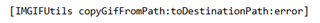
\includegraphics[width=\linewidth]{copyGif_Utils_Line}
  \caption{A utility method called by iMessage after a message has been received but before the message is shown.}
  \Description{A line of code.}
\end{figure}

This line invokes the systems surrounding vulnerability. “Under the hood it uses the CoreGraphics APIs to render the source image to a new GIF file at the destination path.” ~\cite{used_eighth(5)} This isn’t necessarily an issue, but at the time, the implementation performed this step outside of BlastDoor. “BlastDoor isolates, parses, transcodes, and validates untrusted data arriving in Messages, IDS and other vectors to help prevent attacks.” ~\cite{used_ninth(6)} Before rendering occurs, it is necessary to determine the image’s filetype and parse it. Surprisingly, this process does not use the file extension. “The ImageIO library, as detailed in a previous Project Zero blogpost, is used to guess the correct format of the source file and parse it, completely ignoring the file extension.” ~\cite{used_eighth(5)} And it is this flexibility that makes exploit possible. There are known vulnerabilities when parsing PDFs, so Pegasus sends a PDF disguised as a .gif and exploits these vulnerabilities to gain access to the system.
\subsection{PDFs and JBIG2}
NSO uses a PDF disguised as a gif to access vulnerabilities in the PDF parser implementation contained within Apple’s CoreGraphics API. PDFs have supported a compression technique known as the JBIG2 standard since the late 1990’s. JBIG2 allows for extreme compression when working with images containing only black and white pixels. Most of the PDF parser logic within CoreGraphics was Apple proprietary code. But their JBIG2 parsing logic used the open source Xpdf toolkit as part of their implementation. NSO used the extreme compression capabilities of JBIG2 which are supported by two main features.
\subsubsection{Segmentation and Substitution}
A “glyph” is a collection of repeating letters within a text document. JBIG2 attempts to break text documents into segments – glyphs. “The compression algorithm is to simply substitute all sufficiently-similar looking regions with a copy of just one of them” ~\cite{used_eighth(5)}

\begin{figure}[h]
  \centering
  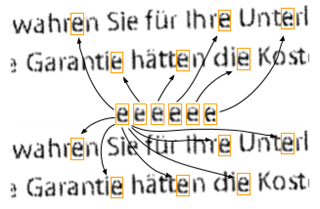
\includegraphics[width=\linewidth]{glyph_visualization}
  \caption{A visualization of parsing a "glyph".}
  \Description{two regions of text with lines drawing a connection between similar letter patterns within each.}
\end{figure}

By replacing all similar glyphs within a text document with a reference to a single compressed version of that glyph, we compress the information greatly. Recreating the text document is as simple as inserting the uncompressed glyph into all recorded locations which contained the same glyph pattern. Like many compression algorithms, there is some risk involved. “There's a significant issue with such a scheme: it's far too easy for a poor encoder to accidentally swap similar looking characters, and this can happen with interesting consequences.” ~\cite{used_eighth(5)}
\subsubsection{Refinement Coding}
The previous technique is lossy, but JBIG2 also supports less-lossy and lossless compression algorithms. “It does this by also storing (and compressing) the difference between the substituted glyph and each original glyph. Here's an example showing a difference mask between a substituted character on the left and the original lossless character in the middle” ~\cite{used_eighth(5)}

\begin{figure}[h]
  \centering
  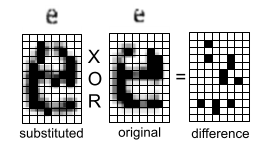
\includegraphics[width=\linewidth]{substitute_char_visualization}
  \caption{difference mask between a substituted character on the left and the original lossless character in the middle.}
  \Description{Three images of character representations. Left, middle, and right.}
\end{figure}

By storing this difference and reapplying it with a logical operator, the loss can be managed. Due to the use of logical operators in this process, JBIG2 streams, which can be thought of as a collection of drawing commands, support the use of most logical operators through this process of “refinement”. “Rather than completely encoding the entire difference in one go, it can be done in steps, with each iteration using a logical operator (one of AND, OR, XOR or XNOR) to set, clear or flip bits. Each successive refinement step brings the rendered output closer to the original and this allows a level of control over the "lossiness" of the compression. The implementation of these refinement coding steps is very flexible and they are also able to "read" values already present on the output canvas.” ~\cite{used_eighth(5)} As we will see later, this is crucial for the exploit.
\subsection{CoreGraphics Parser Vulnerability}
By sending a pdf as a .gif, NSO was able to trigger the JBIG2 decoder within the CoreGraphics stack. By handcrafting the JBIG2 stream embedded within a PDF, they caused an integer overflow to occur within Apple’s PDF parser implementation. NSO used this overflow to set the value of a local variable to something small and exact. This variable is later used to allocate a buffer on the heap. Data is then written to this undersized buffer later in the implementation. Generating a small buffer to work with is essential. If the buffer was allocated with the appropriate size, it would be impossible to write past the end of the buffer.
\subsection{Tying it all Together}
In the next few sub-sections we will see how the tools for implementing such a powerful compression technique and the CoreGraphics PDF decoder implementation paired with deep knowledge of a system and a great capacity for precision allowed NSO trick a simple feature into an unexpected process, gain access to remote regions of memory, build a basic computer architecture from scratch, run a custom scripting language on said computer architecture, and ultimately install their custom spyware Pegasus onto any IOS device without needing the user of that device to do a single thing.
\subsubsection{Buffer Overflow Exploit}
After doctoring the value of a local variable to be small to affect the size of a dynamically allocated heap buffer, NSO write past that buffer to access a JBIG2Bitmap object. NSO will use that bigmap as a playground. By manipulating that bitmap in precise ways, they will be able to construct the necessary logic to install their spyware, but first they must deal with the inevitable crash which would ensue from a standard buffer overflow. “To avoid that crash the heap is groomed such that the first few writes off the end of the syms buffer corrupt the GList backing buffer. This GList stores all known segments and is used by the findSegments routine to map from the segment numbers passed in refSegs to JBIG2Segment pointers. The overflow causes the JBIG2Segment pointers in the GList to be overwritten with JBIG2Bitmap pointers at (4).” ~\cite{used_eighth(5)}

\begin{figure}[h]
  \centering
  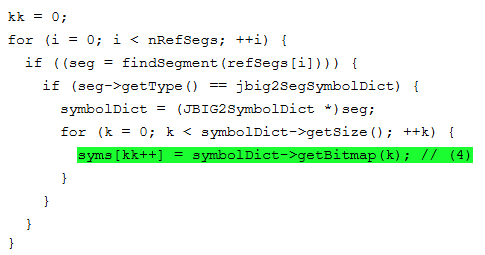
\includegraphics[width=\linewidth]{code_snipit_(4)}
  \caption{A nested loop within Apple's CoreGraphics JBIG2 parser implementation.}
  \Description{A screenshot of code.}
\end{figure}

Before you can write to this undersized buffer, there is a conditional statement checking for type correctness. By rewriting the contents of the Glist backing buffer with JBIG2Bitmap pointers, they prevent further write operations (which would result in a crash) while simultaneously allowing the conditional check to run without errors. It was essential that BOTH issues were handled correctly to avoid a crash.
\subsubsection{Boundless Unbounding}
NSO needs room to work. They accomplish this by something referred to as Boundless Unbounding. “Directly after the corrupted segments GList, the attacker grooms the JBIG2Bitmap object which represents the current page (the place to where current drawing commands render).” ~\cite{used_eighth(5)}

\begin{figure}[h]
  \centering
  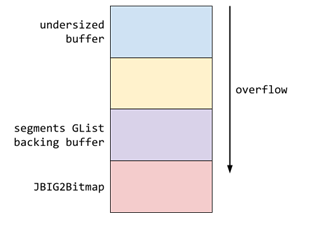
\includegraphics[width=\linewidth]{overflow_to_JBIG2Bitmap}
  \caption{A visualization of the buffer overflow as it passes the Glist backing buffer and reaches a JBIG2Bitmap}
  \Description{Visualization of computer memory during a buffer overflow.}
\end{figure}

The goal is to use the “current page” as a workshop. JBIG2Bitmaps are mostly wrappers around a backing buffer representing a canvas for drawing commands. NSO wants to use this canvas for their own drawing commands. “By carefully structuring refSegs they can stop the overflow after writing exactly three more JBIG2Bitmap pointers after the end of the segments GList buffer. This overwrites the vtable pointer and the first four fields of the JBIG2Bitmap representing the current page.” ~\cite{used_eighth(5)}

\begin{figure}[h]
  \centering
  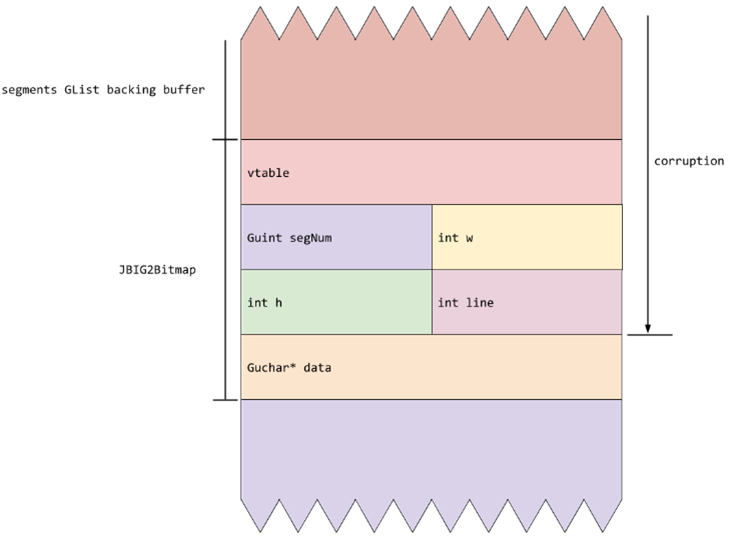
\includegraphics[width=\linewidth]{JBIG2Bitmap_memory_layout}
  \caption{A visualization of the memory of a JBIG2Bitmap object.}
  \Description{Visualization of computer memory during a buffer overflow.}
\end{figure}

During these writes, the original values are being replaced by pointer values. And due to the hardware of the IOS devices, it is easy to predict what those values will be. “Due to the nature of the iOS address space layout these pointers are very likely to be in the second 4GB of virtual memory, with addresses between 0x100000000 and 0x1ffffffff.” ~\cite{used_eighth(5)} With a little forethought, it is possible to doctor the values held by the page height value “h” with very large value. “Since that h value is used for bounds checking and is supposed to reflect the allocated size of the page backing buffer, this has the effect of "unbounding" the drawing canvas. This means that subsequent JBIG2 segment commands can read and write memory outside of the original bounds of the page backing buffer.” ~\cite{used_eighth(5)} During this process NSO was also adjusting the pointer to the page’s backing buffer so that after unbounding, it would be able to read and write to its own fields. This means that by rendering bitmaps to the correct page coordinates, the height, width, and line values can be set to precise values and used to access memory at arbitrary offsets from the backing buffer.

\begin{figure}[h]
  \centering
  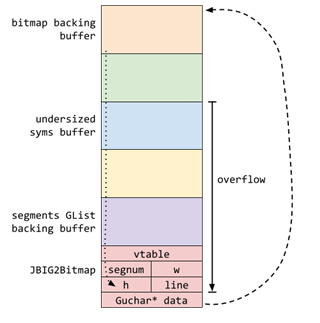
\includegraphics[width=\linewidth]{visualization_of_corruption_after_buffer_overflow}
  \caption{A visualization of the corrupted memory after the buffer overflow.}
  \Description{Visualization of computer memory during a buffer overflow.}
\end{figure}

With just this, NSO could set arbitrary offsets to try and access critical memory locations. This would be a very direct way to gain more influence on the system. But this requires knowing where critical memory locations are.
\subsubsection{Logical Operators}
Now NSO has access to a canvas which they can perform JBIG2 refinement operations on. All logical operators previously mentioned in the \textit{refinement coding} subsection can be used within this unbounded canvas. These operators are normally used within the JBIG2 framework to manipulate pixel data during image refinement, but what else could they be used for? With the ability to access memory at arbitrary offsets from the BIG2Bitmap’s backing buffer, NSO can use these operators on regions of memory within their unbounded range.

\begin{figure}[h]
  \centering
  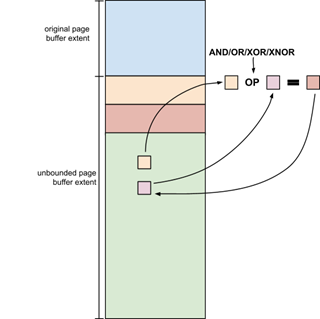
\includegraphics[width=\linewidth]{unbounded_range_visualization}
  \caption{A visualization of how writing to arbitrary locations in memory is possible after unbounding a JBIG3Bitmap.}
  \Description{Visualization of computer memory after unbounding an object through a buffer overflow.}
\end{figure}

NSO uses these operators and the unbounded canvas generated by previous corruption to simulate a logical environment in which to house computational functionality. At this point, the door is open, NSO just needs to step inside and get to work. “JBIG2 doesn't have scripting capabilities, but when combined with a vulnerability, it does have the ability to emulate circuits of arbitrary logic gates operating on arbitrary memory. “ ~\cite{used_eighth(5)} Regardless of the possibility, exploiting this opportunity is still no easy task. “Using over 70,000 segment commands defining logical bit operations, they define a small computer architecture with features such as registers and a full 64-bit adder and comparator which they use to search memory and perform arithmetic operations.” ~\cite{used_eighth(5)} Over the course of a single JBIG2 decompression pass, and through the creative re-purposing of refinement step operations, NSO was able to create a logical framework upon which to operate. The bootstrapping programs build for this FORCEDENTRY exploit are built to run on this rudimentary logical architecture. “It's not as fast as Javascript, but it's fundamentally computationally equivalent.” ~\cite{used_eighth(5)}
\section{Ethical Analysis and Conclusion}
Now we will decide if it is ethical for a government or public agency to spy on a population without their consent in the interest of national security. We will view this question through a specific ethical framework, and then I will draw a conclusion based on that analysis.
\subsection{Act Utilitarianism Lens}
I will use Act Utilitarianism to analyze the question at the center of this paper. I believe the process of trying to understand the impact of non-consensual surveillance through the principle of utility will be enlightening and highlight many of the semantics involved.
\subsubsection{Intensity}
Surveillance takes different forms. In the case of Pegasus spyware, the magnitude of its effect is potentially global. At this point we must make a choice about how to judge the intensity of the surveillance without consent. Due to the likelihood of products like Pegasus being the main tool for enacting surveillance, I am going to judge the intensity based on Pegasus; extreme.
\subsubsection{Duration}
Spying on a population is not an event with a deadline. Pegasus is proof that spyware can be designed to operate indefinitely. There are limits which could impose an indirect duration. If many smart devices were compromised, Pegasus's ability to operate would effectively disappear. But given the likelihood that such an event would take place, I think it is reasonable to say that no, spying on a population does not have a duration.
\subsubsection{Certainty}
The intelligence industry is not a new concept. For the entirety of our history, humans have been spying on each other and gathering intelligence to base their decisions on in many indirect ways. Certainty is 100\%.
\subsubsection{Propinquity}
Spying on someone is an extremely personal and immediate action. When it comes to spyware like Pegasus, it is the personal smart device which is being used to spy, which in some ways, is as close as you can get to a person in space. The surveillance itself is instantaneous. Also with Pegasus, there isn't a delay between when you attempt to spy on someone and when the spying takes place. Propinquity is nearly 100\% in both space and time.
\subsubsection{Fecundity}
Gathering intelligence will most definitely expand the capacity to spy. There are a few essential elements required to pursue anything in this world. Information is absolutely one of them. There is no obvious limit to the amount of useful information that can be obtained or used. It is up to us humans to decide when we should stop.
\subsubsection{Purity}
Spying itself is not a clear director of pleasure or pain. These feelings result from actions taken by humans. Surveillance provides new information that humans can use to make decisions and take actions. But the purity of surveillance is mainly neutral. This follows in part from the fact that surveillance is not meant to be recognized by those being spied on.
\subsubsection{Extent}
This is a tricky one, although potentially billions of people could be spied upon, it is entirely possible that the actors responsibly choose to do nothing with the information they obtain. On the flip side, after spying on a single individual, a decision might be made that would impact potentially millions of people. The extent of non-consensual surveillance is unclear.
\subsection{Conclusion}
Is it ethical for a government or public agency to spy on a population without their consent in the interest of national security? My conclusion is “No”. I present my argument below.
\subsubsection{Purity and Offense vs Defense}
Offense is the best defense, right? In the modern day global geo-political sphere, this concept expresses itself in many ways. Mass surveillance enables transnational repression, which is an act of “authoritarian governments targeting dissidents, journalists and activists outside of their sovereign borders to silence dissent.” ~\cite{used_eighth(5)} Pegasus, the main tool for surveillance being analyzed in this paper, is no exception to this rule. “Lama Fakih, Crisis and Conflict director and head of the Beirut office at Human Rights Watch, was targeted with Pegasus spyware five times between April and August 2021.” ~\cite{used_tenth(11)} Not only does the ability to spy on a population allow you to practice transnational repression, but it also provides the option to cripple said populations ability to heal from any acts of oppression enacted upon it. There are an infinite number of ways for a group of people to be harmed. It is impossible to prepare for all of them. It is up to us to choose where to direct our efforts, and to try and minimize immediate harm in our attempts to prevent future harm. However, we have not made a good name for ourselves in this respect. “The UN Human Rights Council has indeed recognised that many states have used antiterrorism powers as a cynical legal pretext to curtail freedom of expression, legitimise torture and other ill-treatment, and exert a chilling effect on minorities, activists, and political opposition.” ~\cite{used_eleventh(12)} In fact, it seems we are promoting not only immediately harmful acts, but actively seeking ways to tear down our own tools and systems designed for societal self-reflection. “Along with journalists, Pegasus revelations confirm that human rights defenders are one of the key targets being subjected to secret surveillance.” ~\cite{used_twelfth(13)} In the face of mass surveillance having relatively neutral Purity, we have shown as agents of the tool, to strongly push for actions which cause immediate harm without being able to calculate the future harm we might be preventing.
\subsubsection{Propinquity and Privacy}
There are ways to gather information which could help you defend against national threats that are less invasive and less powerful than Pegasus-like spyware. If those less invasive methods were the only players in this game, the act of spying on a population would be less psychologically damaging. But Pegasus is a fundamental part of the spyware industry, and this has a clear effect on the populations being spied on. “Short of not using a device, there is no way to prevent exploitation by a zero-click exploit; it's a weapon against which there is no defense.” ~\cite{used_eighth(5)} Without beating around the bush, for most human beings, knowing that your primary connection to the world is being constantly monitored means a huge portion of your personal life is exposed. This introduces a huge happiness deficit for most people, which probably greatly outweighs the comfort they get from knowing that surveillance might help to prevent some kind of abstract threat to their society.
\subsubsection{Ethical Summary}
At the end of the day, we all make a choice. To form an ethical framework, we must decide what we value. Similarly, when it comes to the question of mass non-consensual surveillance, we must make a choice. What aspects of this question will we focus on? How much value will we give each limb of our analysis? If you decide that you value consistency, then all the “workable” ethical frameworks we have discussed in class would be considered valuable and useful for helping to analyze the ethics of many situations. But let's say you don't value consistency. Let's say you and/or your surrounding society values inconsistency, chaos, and observing each moment without predisposition. In this case, all the “workable” ethical frameworks we have covered would be considered useless, and harmful because the goal of a “workable” ethical framework is to be reusable because of its consistency. I was forced to make a choice. I chose to view this question through the lens of Act Utilitarianism. This does not mean that I have found the answer to the question at heart. It means I have found a way to analyze it, and that analysis resulted in the claim that non-consensual surveillance in the interest of national security is unethical.
\section{Beyond the Superficial}
We must not forget we play a role as in this world, and our actions, no matter how small, influence difficult global issues such as mass surveillance.
\subsection{The Role of a CS Major}
There may not have been any ill intent behind the development of Pegasus, but the products, systems, and tools we bring into the world will undoubtedly be used by others. It is up to us to be aware of this. Technical providers in the industry must recognize that their products can most likely be used for harm. Ideally, business professionals in the industry would invest in defensive capabilities and safeguards before releasing a new product onto the market. Dangerous actors will always exist and will always try to push their own agendas. It is up to the technical people of this world to understand this about reality. “Furthermore, as major US technology companies like Apple and Microsoft began automatically encrypting user communications in recent years, government agencies have sought alternative tools to bypass encryption.” ~\cite{used_thirteenth(14)} Compared to the space of all potential national threats, the space of misuse for a piece of software is manageable. If computing professionals don’t put energy into developing defensive restrictions before releasing their products, the alternative is to try and heal the damage after it’s done. After witnessing how the damage caused by Pegasus was handled, it seems unlikely this will be effective. “Not one victim of spyware abuse has been awarded justice. Not one government has really been held accountable.” ~\cite{used_fourteenth(15)}
\subsubsection{Reflections of a DigiPen Student}
PDFs are such a benign concept. Who would have thought that one day, a person, or multiple people would be harassed or murdered due to a semi-sloppy implementation of a PDF parsing tool. It's bizarre, but I think it suggests a brilliant point. Anything is possible, threats do not exist just because you can't foresee them. Specifically, I have been reminded as I've studied the inner working of Pegasus that a computer is an open playground. We might try to simulate laws or rules, but each one of them is still just a creation of our own logic. And logic can be unwound.
\bibliography{bibliography}{}
\bibliographystyle{ACM-Reference-Format}
\end{document}